\documentclass[aip,amsmath, reprint, author-year]{revtex4-1}
\usepackage{url}
\usepackage[utf8]{inputenc}
\usepackage{hyperref}
\usepackage{graphicx} % for graphics
%\usepackage{listings} % for code listtings
%\usepackage{color}

%\setcitestyle{round, author-year}

\setcounter{page}{1}

%\bibliographystyle{aipauth4-1.bst}

\begin{document}

\begin{abstract}
A approach to generate Generalised Process Capability Data in order to populate and add functionality to a Process Capability Database.
A description of the concept of generalisation, uses and implementation.
\end{abstract}

\title{Concept of using General Process Capability Data}
\author{Andreas Bruun Okholm, s082562\\
Mathias Rask Møller, s082536 }
\affiliation{Technical University of Denmark}
 
\date{\today}
\maketitle

%Introduction

A Process Capability DataBase (PCDB) is a tool for mechanical designers to get information of what is possible to achieve in the companies production. This is done by storing and displaying statistical information about features on produced components.  
By applying Process Capability (PC) information in the design process it is possible to reduces: rework, cost, failure rate, assembly problems and increases product performance \citep{tata1999process}.

As mentioned in \citep{tata1999process, tata1999effective, raskokholm} and a number for key challenges has to be addressed to expand the use of PCDB.
\begin{itemize}
	\item Data Communication: The databases are typically not easily searchable which makes it very difficult to find the correct data and in many cases the data sought after data does not exists. Further more the data is not presented in a way which is easily understandable by mechanical designers.
	\item Fragmented Organization: Development department are dependent on data from production. 
	\item Information Technology: Make a database which is fast, live, global, self populating, up to date and live up to the industry criteria of security and anonymity.
\end{itemize}

There has been a couple of attempts in academia to solve some of these difficulties \citep{thornton2000use, kern2003forecasting, thornton2004variation}, but there hasn't much attention on the subject since indicating there is still issues to resolve before it can be efficiently used in the industry.

In this article we present a concept of data indexing, processing and presentation which tries to make it faster and easier for the mechanical designer to efficiently use process capability data in new designs. 
The general principle is to provide a interface where the data is presented in a much more generalised than typically done in PCDB interfaces. 
The core indexing scheme is simplified, but details are retained or improved using a flexible tagging system. 
Instead of presenting the designer with statistical information, actual recommended specifications limits is shown directly. 
The specification limits is normalised in regards to the specified dimension making more use out of each dataset, minimising the risk of database queries not returning any results. 

Combined with advances in Information Technology we hope this will help make PCDBs a viable tool in the mechanical design process. 

\section{Indexing}
PCDB data needs to be indexed to efficiently retrieve data of relevance to the current design. The data stores in a PCDBs are typically measurements sets; the statistical result of number of measurements of a given part dimension combined with the design characteristics design. Feature, geometry, material and process is suggested by \cite{kern2003forecasting} to be the primary Design Characteristics (DC). For each primary DC there exists a tree structure of possibilities. An example of an index using Kerns proposed design index could be "Plane", "Position", "Aluminium", "Turning". 

In some of the most used processes for mass produced parts like casting and injection moulding, it seems feature and geometry is not necessarily important DCs. The CAM machine milling the moulds does not recognise different features and does not adjust it's precision automatically (SOURCE?).

For our index,  \emph{material} and \emph{process} should be only required DCs. This is combined with a tagging systems, where tags also lives in tree structures. Using tags gives more flexibility since more than one tag can be applied to one measurement set and it's possible to index for design characteristics that's specific to a single production method or material. As an example for injection moulding it would be interesting to index the material type of the mould - aluminium, steel, hardened, ... Indexing the mould iterations (T0, T1, T2) could also give valuable insights about, which specification limits requires mould rework or process adjustment. A last example could to tag if the dimension measured across a parting line in the mould potentially showing a general increase in desired specification limits.

Most product specifications are just plain tolerances (SOURCE?)- these are all just variations of point to point measurements and can as such just be combines into one pool - diameters, positions, thickness, radii... ?

What is measured and since indexed limits the possible conclusions, which can be mades when extracting the data. If the goal is to understand the long term process capability impact of an injection mould process it's either necessary to have measurement sets from many products at different stages of their lifespan or multiple measurements through  the lifespan of a couple of products.    


\section{Processing Capability Data}

Processing the capability data consists of three steps: 

\begin{enumerate}
	\item Compute Process Capability Specification Limit (PCSL).
	\item Normalize PCSL.
	\item Interpret normalised PCSL data.
\end{enumerate}

\subsection{Process Capability Specification Limit}
The process capability indices ($C_p$ and $C_{pk}$) described by \cite{kane1986process} has been widely adopted in statistical process control, been extended and further researched for better understanding \citep{wu2009overview}. 
Instead of looking at process mean $\mu$, standard deviation $\sigma$ and specification upper and lower limits $USL$, $LSL$ using Process Capabilities Indices (PCIs) transforms these values into unit less numbers, which provides a quick overview of how a process is performing.

The PCIs ability to transform process variables of any object into unit less capability index can be reversed to calculate desirable specification limits. For en example the commonly used CPI $C_pk$ 
\begin{equation}
	C_{pk} = \frac{d - | \mu - m|}{3 \sigma}
\end{equation}
can be reversed
\begin{equation}
	d = 3 C_{pk} \sigma + | \mu - m|
\end{equation}
where $d = (USL - LSL) / 2$ is half the specification limit and $m = (USL + LSL) / 2$ is the midpoint between the specification limits. The half specification limit (symmetric tolerance value) is the required tolerance to achieve the desired process capability index value. 

There are several commonly used PCIs each serving their purpose \citep{wu2009overview, taguchi1986introduction}
\begin{itemize}
	\item $C_a$ : Closeness of process mean to target 
	\item $C_p$ : Relative size of variation
	\item $C_{pk}$ : Amount of nonconforming (\%NC)
	\item $C_{pm}$ : Value loss (Taguchi loss function)
	\item $C_{pmk}$: Version of $C_{pm}$,  sensitive to mean shift. 
\end{itemize}

Visualising the $CPIs = 1$  shows how a process on target $C_a = 1$ allows the same variation for all PCIs see figure \ref{fig:CPI}. The line for $C_{pm}$ is in below that of $C_{pk}$ except for values of $C_a$ close to 1. 
Using $C_{pm}$ will in general be more conservative resulting in larger specification limits than $C_{pk}$. The plot shown is for a capability equal to one for higher values this effect is even more pronounced.

\begin{figure}
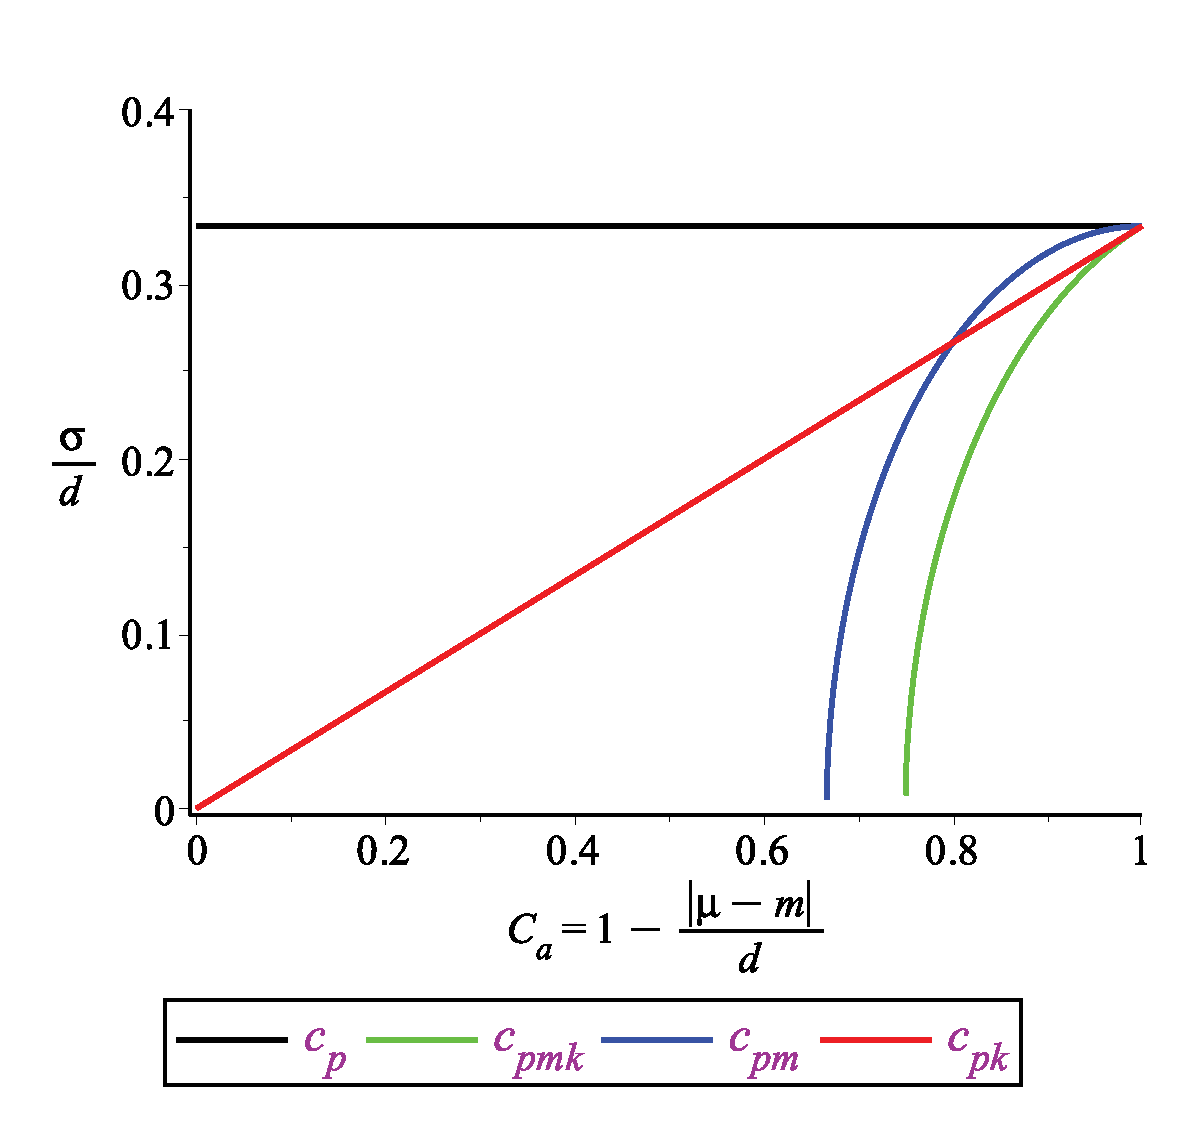
\includegraphics[width=0.45\textwidth]{graph_postscript_test.eps}
\caption{\label{fig:CPI} $C_p$ referens only to the variance of the process. $C_{pk}$ is related to the yield of the product. $C_{pm}$ takes a loss function in to account relates to a target dimension. $C_{pmk}$ takes both the yield of the product and a loss function. }
\end{figure}

For the purpose of our database we have chosen to use $C_{pk}$, since it provides the most easily understandable result - directly related to the yield of the process. The yield of a process is within $2\Phi(3C_{pk})-1 \leq \text{yield} < \Phi(3C_{pk})$ where $\Phi(\cdot)$ is the cumulative distribution function of the standard normal distribution N(0,1) \citep{boyles1991taguchi}. For typical capability levels the resulting non-conforming products in parts per million (ppm) is listed in table \ref{tab:cpl_nc}

\begin{table}
\begin{ruledtabular}
\caption{\label{tab:cpl_nc} $C_{pk}$ Non-conformaties}
\begin{tabular}{llll}
  $\mathbf{C}_{pk}$	& $\sigma$ level	& $\mathbf{NC_\mathrm{max}} \mathrm{\ (ppm)}$	&  $\mathbf{NC_\mathrm{min}} \mathrm{\ (ppm)}$	\\
  1.00	& 3		& 2699.8		& 1349.9		\\
  1.33 	& 4 		& 63.3		& 31.7 		\\
  1.50 	& 4.5 	& 6.7		& 3.4		\\
  1.66	& 5		& 0.6		& 0.3		\\
  2.00	& 6		& 0.002		& 0.001		\\
\end{tabular}%
\end{ruledtabular}
\end{table}

CONCLUDE ON WHAT CPK LEVEL TO USE

Using $C_{pm}$ would be sensible sense if the desired tolerances directly influence product performance - for instance in optics construction.  


\subsection{Normalization}
Comparison of different standard tolerance dimension relations. 

ISO 286? describes a non-linear function for comparing tolerances on objects of different dimension. This function used to normalize tolerances and display PC independent of size (with in the limits of the function.)  

Tysk og fransk standarder plast støbe standarder
finde kilder

ANSI ?!

Choice of ISO based continious function and customary user in industry

\subsection{Analyze normalized data}



fit normal distribution of sub groups.
find subgroups

extracting data

robustness 



visible confidence intervals of interpertation


\section{User Interface}

Readability of accumulated normal distribution compared to a bell curve.

Two figures showing the actual interface

General
	Interactivity in plots 
		Special courses comment of measurement sets.
	
	Group sorting
		Reference to Thornton graphical display article.

	Visible confidence intervals

	User can set tolerance (from IT to specific dimentions)

Two views
	General charts inspired by ANSI
	Process view inspired by Thornton Graphical display


\section{Statistical Validity}

measurement sets are assumed to fit a normal distribution.

What you measure is what you get.
Each product in the sample set, produces a measurement. From the sample set is a  measurement set created. 

Confidence intervals - sample size of each measurement set.

\begin{figure}
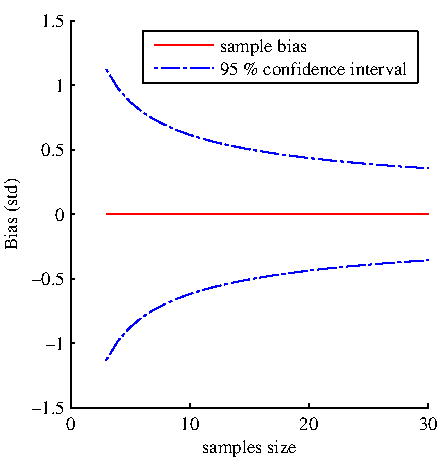
\includegraphics{stats_bias_confidence.pdf}
\caption{\label{fig:std_uncertainty}The uncertainty of the standard deviation estimate is reduced as the number of samples is increased. The increase in accuracy gained per additional decreases with more samples. From the graph we have chosen 12 to be the optimal point for general process capability use.}
\end{figure}

\begin{figure}
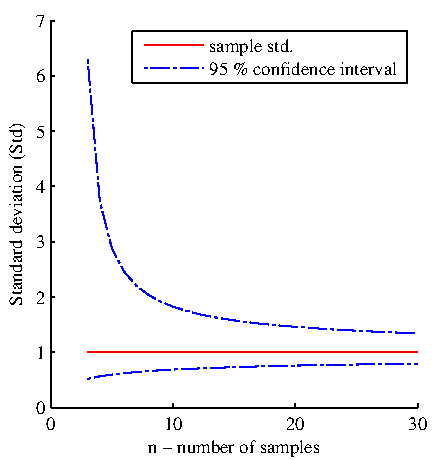
\includegraphics{stats_std_confidence.pdf}
\caption{\label{fig:std_uncertainty}The uncertainty of the standard deviation estimate is reduced as the number of samples is increased. The increase in accuracy gained per additional decreases with more samples. From the graph we have chosen 12 to be the optimal point for general process capability use.}
\end{figure}

Number of measurement sets to predict process capability.  


show current production capability in terms of it-grade

\section{Using the general process capability data}
apply tolrance, By looking at normalized data of the variance of products of the same material and process, it is possible to find a suitable tolerance
improvement per rework
material selection


\section{Discussion}

Using todays techonolgy, generalization of PC data upon request from the user i feasble. A proposed techincal setup is described in \cite{OkholmRask}.

Initiating PCG is a tough process. 
The reward for doing robust design engineering is long reach
The reward for using PCDB or robust design in general to make changes in early design is a long term and might only benefit the company and not feedback to the designers compared the reward for the hero in production solving the expensive errors in design.

Implementing GPC requires a change
	economical barrier
		big company
			incement from quality department
			gain: 	knowlegde of own PC
					high precision data
					Extensive knowlegde on causes and problem
			loss:
		cross companies
			diverse data
			gain:		Alot of data
					knowlegde of processes and matrial outside your field
					knowlegde of possible to achive in industry
					Index storing of own data and partially analysed
			loss:		Indusry espiange concerns
					loss of information due to anonymity

proto running at a university, unbiast.


\section*{References}
\bibliography{../PCDBmasterBibliography/PCDB_Master_bib.bib}

\end{document}